%\myChapter{Titre}{Titre court}
\myChapter{état de l'art sur les politiques et modèles de contrôle d'accès}{}
\label{chapEtatDeLart}
%\myMinitoc{Profondeur de la minitoc (section|subsection|subsubsection)}{Titre de la minitoc}
\myMiniToc{section}{Sommaire}

\mySubSection{Introduction}{}\label{sectionIntroduction}

La sécurité des systèmes d'information a pour but de garantir trois propriétés fondamentales appelées objectifs de sécurité : la confidentialité, l'intégrité et la disponibilité. La confidentialité assure que seules les personnes autorisées peuvent accéder à une information. L'intégrité, quant à elle,  vise à empêcher toute altération ou destruction d'une information par des personnes malveillantes. La disponibilité garantit que l'information est accessible aux personnes autorisées quand elles en ont besoin. De ce fait plusieurs méthodes de sécurité telles que le contrôle d'accès ont été proposées. Le contrôle d'accès a pour but de limiter les actions ou les opérations qu'un utilisateur légitime du système informatique peut effectuer. Faisant l'objet de nombreuses recherches plusieurs approches de contrôle d'accès plus connues sous le nom de modèle de contrôle d'accès ont été implémentées. Parmi ces modèles, nous pouvons citer : DAC (Discretionary Access Control), MAC (Madatory Access Control), RBAC (Role Based Access Control), Or-BAC (Organization Based Access Control), ABAC (Attribute Based Access Control) et HOr-BAC (Hierarchy Organization Based Access Control).

\paragraph{} Dans ce chapitre, nous définirons d'une part quelques notions de base de la sécurité des systèmes d'information, et d'autre part nous présenterons les différents modèles de contrôle d'accès ainsi que leurs avantages et leurs inconvénients.



%SECTION TRAVAIL COOPERATIF
%\mySection{Titre}{Titre court}
%\mySection{Définition de Quelques notions de la sécurité des systèmes d’information}{}\label{sectionDédinitionNotions}
%Le terme...
%\begin{preuve}
%La preuve
%\end{preuve}

%\begin{example}\textit{Le cultivateur et son champ}\\
%Un cultivateur...
%\end{example}

\mySection{Politiques et modèles de contrôle d'accès discrétionnaires (DAC)}{}\label{sectionDAC}

Les politiques de protection discrétionnaires régissent l'accès des utilisateurs à l'information sur la base de l'identité de l'utilisateur et des autorisations qui spécifient pour chaque utilisateur (ou groupe d'utilisateurs) et chaque objet du système, les modes d'accès auxquels l'utilisateur est autorisé à effectuer sur l'objet \cite{sandhu94}. Chaque demande de l'utilisateur pour accéder à un objet est vérifiée par rapport aux autorisations spécifiées. S'il existe une autorisation statuant que l'utilisateur peut accéder à l'objet dans le mode spécifique, l'accès est accordé, sinon il est refusé. Le guide NCSC (A Guide To Understanding Discretionary Access Control in Trusted Systems) indique que la base du DAC est qu'un utilisateur individuel, ou un programme fonctionnant au nom de l'utilisateur est autorisé à spécifier explicitement les types d'accès que les autres utilisateurs (ou les programmes s'exécutant en leur nom) peuvent avoir aux informations sous le contrôle de l'utilisateur. Deux propriétés spécifiques caractérisent DAC :\\ 
-La notion de contrôle : il existe une notion selon laquelle les utilisateurs exercent un contrôle sur les ressources, en ce sens qu'un utilisateur qui contrôle une ressource obtient de dicter les sortes de droits que les autres utilisateurs ont sur la ressource.\\
-La notion d'initialisation d'une action par un utilisateur pour changer l'état de protection de tels changements d'état se produisent parce que des utilisateurs particuliers initient de tels changements.\\
Les politiques de contrôle d'accès se basent sur le modèle de matrice d'accès pour la définition des autorisations qu'ont les utilisateurs sur les objets.
\paragraph{} La flexibilité des politiques discrétionnaires les rend adaptés à une variété de systèmes et d'application. Pour ces raisons, elles ont été largement utilisées dans une variété d'implémentations, en particulier dans les environnements commerciaux et industriels.

\mySubSection{Modèle de matrice d'accès}{}\label{sectionMatriceAccès}

La matrice d'accès est un modèle conceptuel qui spécifie les droits que chaque sujet possède pour chaque objet. Cette matrice définit trois types d'entités \cite{rjaibi04} :\\
-Les objets protégés : ce sont les entités ou ressources auxquelles on peut  accéder.\\
-Sujet : ce sont des entités actives qui accèdent aux objets.\\
-Les droits d'accès : qui associent les sujets aux objets protégés, ceci en spécifiant les opérations que les sujets peuvent effectuer sur les objets.
\paragraph{} Dans cette matrice, les lignes représentent les sujets, les colonnes représentent les objets et les cellules représentent des droits qu'ont les sujets sur les objets. La tâche du contrôle d'accès est d'assurer que seules les opérations autorisées par la matrice d'accès sont exécutées. Ceci est réalisé au moyen d'un moniteur de référence qui est responsable de la médiation de toutes les opérations tentées par les sujets sur les objets. De façon générale, le propriétaire d'un fichier est autorisé à accorder aux autres utilisateurs l'accès ou non au fichier \cite{sandhu94}. Le tableau 1 montre un exemple de matrice d'accès. Dans cette matrice, nous voyons que Bob détient des droits de lecture (R) et d'écriture (W) sur le fichier 1 ; des droits de propriété  (Own), de lecture et d'écriture sur le fichier 3 et le droit d'exécution sur le fichier 4 et n'a aucun droit sur le fichier 2.
\begin{figure}[h!]
    \centering
		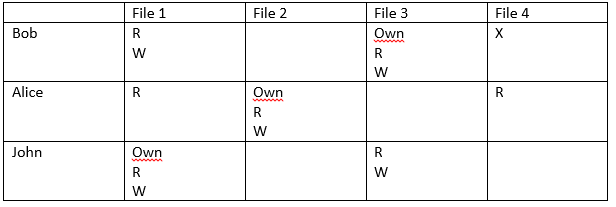
\includegraphics[scale=0.7]{chap2/images/ACM.png}
    \caption{exemple de matrice d'accès}
	 \label{figAcm}
\end{figure} 


\mySubSection{Implémentation des politiques discrétionnaires}{}\label{sectionApproche}

Dans de grands systèmes, la matrice d'accès est énorme en taille et la plupart de ses cellules vides, ce qui rend ainsi son implémentation rare. De ce fait en pratique, il est développé plusieurs approches de la matrice d'accès. 


\mySubSubSection{Liste de contrôle d'accès}{}\label{sectionACL}

Une approche populaire de l'implémentation de la matrice d'accès est l'utilisation des listes de contrôle d'accès. Ici, chaque objet est associé à une liste de contrôle d'accès (ACL) qui indique pour chaque sujet du système les accès que le sujet est autorisé à exécuter sur l'objet. Cette approche correspond à un stockage de la matrice par colonnes \cite{sandhu94}. Le schéma 1 ci-dessous illustre les ACL de la matrice d'accès ci-dessus. En consultant l'ACL d'un objet, il est facile de déterminer quels modes d'accès sont actuellement autorisés pour cet objet. C'est-à-dire que, les ACL permettent de vérifier les accès à un objet. Il est également facile de supprimer tous les accès à un objet en remplaçant l'ACL existante par une ACL vide. Par contre, il est difficile de déterminer tous les accès d'un sujet dans un système basé sur les ACL. Car cela nécessite un examen de la liste de contrôle d'accès de chaque objet du système pour faire le contrôle d'accès d'un sujet. De manière similaire, si tous les accès d'un sujet ont besoin d'être révoqués, toutes les ACL vont être visitées une par une. 
\paragraph{} De nombreux systèmes permettent aux noms de groupe d'apparaître dans les listes de contrôle d'accès. Les systèmes d'exploitation tels que l'UNIX et VMS implémentent une forme abrégée d'ACL dans laquelle un petit nombre de noms de groupe, souvent un ou deux, peuvent apparaître dans l'ACL \cite{sandhu94}.

\begin{figure}[h!]
    \centering
		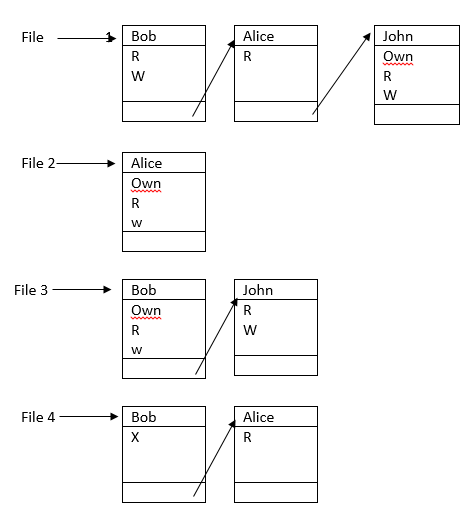
\includegraphics[scale=0.7]{chap2/images/acl.png}
    \caption{ACL de la matrice d'accès ci-dessus}
	 \label{figAcl}
\end{figure}

\mySubSubSection{Les capacités}{}\label{sectionListeCapacité}

Les capacités sont une approche duale des ACL. Ici, chaque sujet est associé à une liste de capacité qui indique, pour chaque objet du système quels accès le sujet est autorisé d'exécuter sur l'objet. Cette approche correspond au stockage de la matrice d'accès par lignes. La liste des capacités permet facilement de voir tous les accès qu'un sujet est autorisé à effectuer, ceci par un simple examen de la liste des capacités. Toutefois, déterminer tous les sujets qui peuvent accéder à un objet revient à un examen de la liste des capacités de chaque sujet. Cette approche, contrairement aux ACL n'a pas connue de succès. Il est possible de combiner les ACL et les capacités. La possession d'une capacité est nécessaire pour qu'un utilisateur obtienne l'accès autorisé par cette capacité. Dans les systèmes distribués, cette approche présente l'avantage de ne pas nécessiter une authentification répétée du sujet. Cela permet à un utilisateur d'être authentifié une seule fois et d'obtenir ces capacités, puis de les présenter pour obtenir des services de la part de plusieurs serveurs du système. Chaque serveur peut en autre utiliser des ACL pour fournir un contrôle d'accès détaillé \cite{sandhu94}.

\mySubSection{Vulnérabilité des politiques discrétionnaire}{}\label{sectionVulnérabilitéDAC}

Les politiques discrétionnaires ne font pas de distinction entre les utilisateurs et les sujets. De façon  générale, les utilisateurs sont des entités passives pour lesquelles des autorisations peuvent être spécifiées et qui peuvent se connecter au système. Une fois connectés au système, les utilisateurs créent des processus (sujets) qui s'exécutent en leur nom et, par conséquent, soumettent des demandes au système. Elles évaluent ainsi toutes les demandes des processus exécutés au nom d'un utilisateur par rapport aux autorisations de l'utilisateur. Cependant une analyse plus précise pour le problème de contrôle d'accès montre une utilité de séparer les utilisateurs des sujets. Un autre inconvénient des politiques discrétionnaires est qu'elles ne fournissent pas une réelle assurance sur les flux d'information dans le système. Par conséquent, il est facile de contourner les restrictions d'accès énoncés dans les autorisations. Par exemple, un utilisateur qui a le droit de lire sur un fichier peut le transmettre à d'autres utilisateurs non autorisés pour le lire sans que le propriétaire du fichier ne soir au courant. Afin de palier à cet inconvénient, les politiques obligatoires ont vu le jour.


\mySection{Politiques et modèles de contrôle d'accès obligatoire (MAC)}{}\label{sectionMAC}

Contrairement aux politiques discrétionnaires, les politiques obligatoires centralisent l'autorité d'administration des droits à un seul utilisateur généralement appelé super-utilisateur \cite{lindqvist06}. Les politiques obligatoires régissent l'accès sur la base de la classification des sujets et des objets dans le système. Les objets sont des entités passives stockant des informations. Les sujets sont des entités actives qui demandent l'accès aux objets. Il est bon à savoir ici que les politiques obligatoires font une distinction entre les utilisateurs et les sujets. Les utilisateurs sont des êtres humains qui peuvent accéder au système, tandis que les sujets sont des processus (programmes en cours d'exécution) opérant pour le compte des utilisateurs. Cette distinction permet à la politique de contrôler les accès indirects (fuites ou modification) provoqués par l'exécution des processus \cite{samarati00}. Dans ce modèle, on associe à chaque sujet et à chaque objet du système un niveau de sécurité. Le niveau de sécurité associé à un objet reflète la sensibilité de l'information contenue dans l'objet, c'est-à-dire le dommage potentiel qui pourrait résulter de la divulgation non autorisée de ces informations. Le niveau de sécurité associé à un utilisateur, également appelé autorisation, reflète la confiance de l'utilisateur dans le fait de ne pas divulguer d'informations sensibles à des utilisateurs non autorisés à les voir. De façon simple, un niveau de sécurité est un élément d'un ensemble hiérarchique ordonné. Les niveaux de sécurité les plus connus sont : très secret (TS), secret (S), confidentiel (C), non classifié (U). Chaque niveau de sécurité se domine lui-même et tous les autres en dessous dans cette hiérarchie, exemple : TS>S>C>U \cite{sandhu94}.
\paragraph{} L'accès à un objet par un sujet n'est accordé que si une certaine relation est satisfaite entre les niveaux de sécurité associés aux deux en particulier, les deux principes suivants doivent être respectés \cite{sandhu94} :\\
-Read down : l'autorisation d'un sujet doit dominer le niveau de sécurité de l'objet en cours de lecture.\\
-Write up : l'autorisation d'un sujet doit être dominée par le niveau de sécurité de l'objet en cours d'écriture.
\paragraph{} La satisfaction de ces principes empêche les informations connues dans les objets de haut niveau (c'est-à-dire plus sensibles) de circuler vers les objets de niveaux inférieurs. Dans un tel système, les informations ne peuvent circuler que vers le haut ou au sein de la même classe de sécurité. Notons, l'importance de contrôler à la fois les opérations de lecture et d'écriture, car les deux peuvent être utilisées de manière inappropriée pour divulguer des informations. Les politiques basées sur ces deux principes permettent de fait la différence entre les utilisateurs et les sujets. En effet à travers le Read down les sujets sont empêchés de lire les informations contenues dans les objets de classe supérieure ; et à travers le principe d'écriture ascendante, elles empêchent les logiciels malveillants de divulguer des secrets vers le bas : de la classe supérieure à la classe inférieure. Ici, on fait confiance aux utilisateurs pour ne pas divulguer de telles informations, mais les programmes qu'ils exécutent ne méritent pas le même degré de confiance. Cette règle empêche également les utilisateurs de divulguer des informations du haut vers le bas.
\paragraph{} Outre les niveaux de sécurité hiérarchiques, les catégories (Par exemple : crypto, NATO, Nucléaire) peuvent également être associées à des sujets et à des objets. Dans ce cas, les étiquettes à chaque sujet et à chaque objet consistent en une paire composée d'un niveau de sécurité et d'un ensemble de catégories. L'ensemble de catégories associé à un sujet reflète les domaines spécifiques dans lesquels les utilisateurs opèrent. L'ensemble des catégories associé à un objet reflète les domaines auxquels les informations contenues dans les objets sont référées. La prise en compte des catégories permet une classification de sécurité plus fine. Elles servent de base à l'application des restrictions liées au besoin de connaissance (c'est-à-dire qu'elles limitent l'accès des sujets aux informations qu'ils ont réellement besoin de connaître pour effectuer leur travail).
\paragraph{} Le contrôle d'accès obligatoire peut également être appliqué pour la protection de l'intégrité des informations. Ici, le niveau d'intégrité associé à un objet reflète le degré de confiance que l'on peut accorder aux informations stockées dans l'objet et des dommages potentiels qui pourraient résulter d'une modification non autorisé de l'information. Le niveau d'intégrité associé à un utilisateur reflète la capacité de l'utilisateur à insérer, modifier ou supprimer des données et des programmes à ce niveau. Des principes similaires à ceux, énoncés pour le secret doivent être respectés comme suite \cite{sandhu94}. : \\
- Read up : le niveau d'intégrité d'un sujet doit être dominé par le niveau d'intégrité de l'objet en cours de lecture. \\
- Write down : le niveau d'intégrité d'un objet doit dominer celui de l'objet en cours d'écriture.
Le respect de ces principes garantit l'intégrité en empêchant les informations stockées dans les objets de niveaux inférieurs de circuler vers les objets de niveaux supérieurs. Le contrôle de flux d'information n'est qu'un aspect de la réalisation de l'intégrité.
\paragraph{} Les politiques mandataires sont implémentées dans les systèmes d'exploitation tels que vista et Linux et elles sont également utilisées dans les bases de données.


\mySubSection{Vulnérabilité des politiques Obligatoire}{}\label{sectionVulnérabilitéMAC}

Bien que les politiques obligatoires offrent une protection contre les fautes d'informations indirectes, elles ne garantissent pas le secret complet de l'information. En effet, les politiques obligatoires de secret ne contrôlent que les canaux manifestent d'information (c'est-à-dire les canaux légitimes). Elles restent toujours vulnérables aux canaux secrets. Il s'agit des canaux qui ne sont pas destinés à la communication normale, mais qui peuvent néanmoins être exploité pour déduire des informations. 
Les politiques mandataires sont lentes à administrer et sont également rigides dans leur fonctionnement. De plus, ils ne permettent pas de contrôler le DBA au sein d'une organisation.


\mySection{Politiques et modèles de contrôle d'accès basés sur les rôles (RBAC)}{}\label{sectionRBAC}

Les politiques discrétionnaires et obligatoires sont difficiles à administrer pour les organisations de grande taille. En effet, dans ces politiques, il faut à chaque fois enregistrer tous les utilisateurs et définir les droits d'accès aux objets du système pour chaque sujet. Les politiques basées sur les rôles  (RBAC) viennent résoudre ce problème en accordant les droits d'accès aux rôles plutôt qu'aux utilisateurs individuellement \cite{sandhu96}. Les politiques basées sur les rôles régulent l'accès des utilisateurs aux informations sur la base des activités qu'ils exécutent dans le système. Ces politiques nécessitent l'identification des rôles dans le système. Un rôle peut être défini comme un ensemble d'actions et de responsabilités associées à une activité professionnelle particulière. Ensuite, au lieu de spécifier tous les accès que chaque utilisateur est autorisé à exécuter, les autorisations d'accès aux objets sont spécifiées pour les rôles. Les utilisateurs reçoivent des autorisations pour adopter des rôles. Une étude récente du NIST confirme que les rôles qui sont une approche utiles pour de nombreuses organisations commerciales et gouvernementales. L'utilisateur jouant un rôle est autorisé à exécuter tous les accès pour lesquels le rôle est autorisé. En général, un utilisateur peut jouer différents rôles à différentes occasions. Certaines propositions de contrôle d'accès basées sur les rôles permettent à un utilisateur d'exercer plusieurs rôles en même temps \cite{sandhu94}. Un rôle qui est principalement une construction sémantique formant la base de la politique de contrôle d'accès. Avec RBAC, les administrateurs du système créent des rôles en fonction des fonctions exercées dans une entreprise ou une organisation, donnent les permissions (autorisations) d'accès à ces rôles, puis affectent les utilisateurs aux rôles en fonctions de leurs responsabilités et qualifications professionnelles spécifiques.

\begin{figure}[h!]
    \centering
		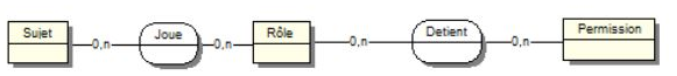
\includegraphics[scale=0.7]{chap2/images/RBACstandard.png}
    \caption{Attribution des permissions aux sujets à travers des rôles}
	 \label{figARbac}
\end{figure}

\mySubSection{Composants principaux de RBAC}{}\label{sectionComposantRBAC}

RBAC est généralement composé des quatre éléments suivants \cite{bellettini01} :

\myDescription{User ou Utilisateur}{un utilisateur est défini comme un être humain, une machine, un réseau, un processus ou un agent autonome intelligent. Cette définition couvre différents domaines de sécurité et des domaines d'application, par exemple : les bases de données.
}

\myDescription{Rôle}{Un rôle est généralement une fonction qui dans le contexte d'une organisation avec une sémantique associée concernant son autorité et sa responsabilité.
}

\myDescription{Permission}{Une permission est un mode d'accès qui peut être exercé sur des objets d'un système. Les objets et les modes d'accès dépendent du domaine. Par exemple, dans le cas d'une base de données, l'ensemble d'objets comprend des tables, des colonnes et des lignes, et l'ensemble des modes d'accès comprennent des opérations d'insertion, de suppression et de mise à jour.}

\myDescription{Session}{Une session est une instance particulière d'une connexion d'un utilisateur au système et définit le sous-système de rôles activés. A chaque instant, différentes sessions pour le même utilisateur peuvent être activées. Lorsque l'utilisateur se connecte au système, il établit une session et pendant celle-ci, il peut demander d'activer un sous-ensemble du rôle qu'il est autorisé à jouer. L'utilisateur obtient toutes les permissions associées aux rôles qu'il a activés dans sa session.}

\begin{figure}[h!]
    \centering
		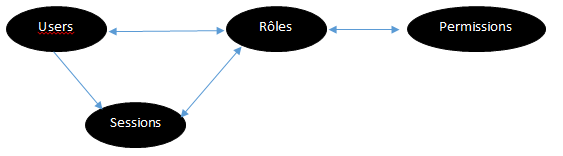
\includegraphics[scale=0.7]{chap2/images/rbac.png}
    \caption{RBAC standard}
	 \label{figRbac}
\end{figure}

\paragraph{} Au fil des années, différentes variantes du modèle RBAC ont été mises sur pieds afin d'introduire de nouveaux concepts tels que la hiérarchie des rôles et la séparation des tâches.

\mySubSection{Hiérarchie des rôles}{}\label{sectionHiérarchieRole}

Les hiérarchies des rôles représentent une amélioration importante du RBAC standard, car elles constituent un moyen naturel de structurer les rôles pour refléter la structure de cette organisation. A cette fin, une relation d'ordre partiel sur les rôles est introduite, appelée hiérarchie des rôles \cite{theseBenoit}. La hiérarchie des rôles, définie comme RHC Rôles × Rôles, identifie l'ensemble des paires de rôles <ri, rj> telles que le rôle ri  hérite du rôle rj. Dans la littérature, il existe deux interprétations différentes de l'héritage :\\
-La hiérarchie générale : elle permet de supporter le concept de hiérarchie multiple qui fournir la capacité d'héritage des permissions de deux rôles ou plus ;\\
-La hiérarchie limitée : elle se base sur les mêmes principes que la hiérarchie générale, cependant elle ne supporte pas l'héritage multiple.

\begin{figure}[h!]
    \centering
		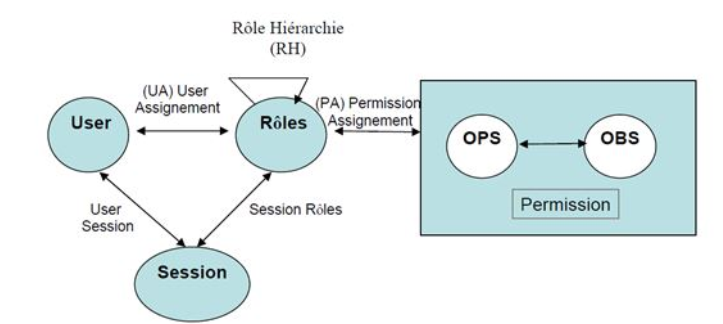
\includegraphics[scale=0.7]{chap2/images/HierachieRole.png}
    \caption{Hiérarchie RBAC}
	 \label{figHrbac}
\end{figure}

\mySubSection{Notion de séparation des tâches}{}\label{sectionSéparationTache}

La notion de séparation de tâches a été ajoutée dans le modèle RBAC. Celle-ci stipule qu'aucun utilisateur ne possède assez de privilèges pour abuser seul du système, afin d'assurer que les fraudes et les erreurs majeures ne peuvent avoir lieu que par une collaboration préméditée de plusieurs utilisateurs. Au sein des organisations, ceci se traduit par le fait d'empêcher l'utilisateur de jouer des rôles conflictuels ou aussi de restreindre le nombre de rôles associés aux utilisateurs d'une façon statique ou dynamique. A cet effet, ce modèle distingue deux types de séparation de tâches \cite{sandhu96} : la séparation statique des devoirs (SSD) vise à empêcher le conflit d'intérêts qui survient lorsque les rôles en conflits sont affectés à un même utilisateur et la séparation dynamique des devoirs (DSD) qui impose le contrôle dynamiquement par une contrainte sur les rôles lors de l'activation d'une session donnée.


\mySubSection{Avantages du modèle RBAC}{}\label{sectionAvantageRBAC}

L'approche d'un contrôle d'accès basée sur les rôles présente des avantages incontestables sur différents plans \cite{theseBenoit}:

\myDescription{Gestion des autorisations}{Les politiques basées sur les rôles bénéficient d'une indépendance logique dans la spécification des autorisations des utilisateurs en divisant cette tâche en deux parties. L'une attribue les utilisateurs aux rôles et l'autre attribue les droits d'accès aux objets aux rôles. Cela simplifie grandement la gestion de la sécurité. Par exemple, supposons qu'un utilisateur change de responsabilités, disons en raison d'une promotion.
}

\myDescription{Hiérarchie des rôles}{Dans de nombreuses applications, il existe une hiérarchie naturelle des rôles, fondé sur les principes familiers de généralisation et de spécification. Exemple : les rôles ingénieurs logiciels et ingénieurs matériels sont des spécifications du rôle d'ingénieur. Un utilisateur affecté à l'un de ces rôles héritera également des privilèges et autorisations attribués aux rôles plus généraux d'ingénieur ; les rôles hiérarchiques simplifient encore la gestion des autorisations.
}

\paragraph{} Le modèle RBAC a été implémenté dans plusieurs systèmes parmi lesquels le système Oracle, Dresdner Bank une banque européenne internationale comportant 50 659 employés et 1459 branches dans le monde dont la branche principale est située en Allemagne.

\mySubSection{Inconvénient du modèle RBAC}{}\label{sectionInconvéniantRBAC}

RBAC a été critiqué dans \cite{abou03} pour les raisons suivantes :\\
- Le concept de hiérarchie de rôle est quelque peu ambigu. En général, la hiérarchie des rôles ne correspond pas tout à fait à la hiérarchie organisationnelle. Par exemple, le directeur de l'hôpital a un rôle administratif supérieur au rôle de médecin. Pour autant, un directeur de l'hôpital n'est pas nécessairement un médecin, ainsi, il n'est pas faisable d'accorder au directeur les permissions du médecin.\\
- Peut utiliser pour les organisations qui suivent les autres modèles à l'instar du modèle réseau. \\
- L'impossibilité d'exprimer des règles contextuelles relatives aux permissions, aux interdictions, aux obligations et aux recommandations et notamment des permissions qui dépendent du contexte. Par conséquent, il serait difficile de spécifier qu'un médecin n'a la permission d'accéder au dossier médical d'un patient que si ce dernier est son patient.

\mySection{Politiques et modèles de contrôle d'accès basé sur les organisations (ORBAC)}{}\label{sectionORBAC}

Aucun des modèles classiques de contrôle d'accès tels que DAC, MAC ou RBAC n'est pleinement satisfaisant pour modéliser des politiques de sécurité qui ne se limitent pas à des permissions statiques, mais incluent également des règles contextuelles liées à des permissions, des interdictions, des recommandations. C'est ainsi qu'Or-BAC a été proposé pour permettre la spécification de telles politiques de sécurité contextuelles. Or-BAC est un modèle de contrôle d'accès basé sur l'organisation \cite{kalam03}. L'organisation représente l'ensemble des rôles, des activités et des vues qui représentent les abstractions respectives des utilisateurs, des opérations et des objets par rapport à une organisation donnée. Par exemple, un utilisateur est lié à un ensemble de rôles pour une organisation donnée. Il peut être affecté à d'autres rôles pour une autre organisation. Or-BAC défini des relations ternaires entre les organisations, les sujets et les rôles : un sujet joue un rôle dans une organisation  \cite{lindqvist06}. Ce qui veut dire que l'utilisateur ayant plusieurs rôles peut activer tous les rôles, soit un sous-ensemble de ses rôles dans n'importe quelle équipe à laquelle il participe. Dans la pratique, même si un utilisateur possède plusieurs rôles, il n'a pas forcément le droit de les jouer dans toutes les équipes auxquelles il appartient \cite{kalam03}.


\mySubSection{Relations existantes entre les entités du niveau concret et les entités du niveau abstrait }{}\label{sectionRelation}

\myDescription{Relation entre les sujets et les rôles}{Dans ce modèle, un sujet est considéré comme étant une entité active du système, c'est-à-dire un utilisateur, soit une organisation. Les exemples de sujet comprennent donc des utilisateurs tels que  Jean, Marie, Pierre Ou des organisations telles que «  le service comptable de la clinique privée langue-Doc, … ». L'entité rôle est utilisée pour structurer le lien entre les sujets et les organisations. Dans le domaine de la santé, les rôles « cardiologue », « infirmière », « médecin » seront joués par des utilisateurs tandis que les rôles « service des urgences », « équipe de secours », « unité de soins intensifs » seront joués par des organisations. Puisque les sujets jouent des rôles dans les organisations, nous avons besoin d'une relation qui relie ces entités ensemble. La relation liant le sujet, le rôle et l'organisation est une relation habilitée. Par exemple, la relation habilitée (FS-UDS, Paul, coordonnateur) signifie «  l'organisation FS-UDS habilite le sujet Paul dans le rôle coordonnateur » \cite{theseBenoit}. La définition des rôles, l'affectation des rôles aux sujets et l'héritage des permissions à travers la hiérarchie ont pour objectif de structurer l'ensemble des sujets d'une organisation et de simplifier ainsi la gestion de la politique de sécurité.
}

\myDescription{objets et vues}{Les objets Or-BAC représentent des entités passives (fichiers, dossiers, administratifs, dossiers d'inscription, fichiers de note). Une vue correspondant à un ensemble d'objets qui satisferont une propriété commune (comme dans une base de données relationnelles) par exemple dans un système de gestion de fichiers, la vue « dossiers administratifs » correspond aux dossiers administratifs des patients alors que la vue « dossier médical » correspond aux dossiers médicaux des patients... Par conséquent, une relation appelée utilise est définie pour relier les organisations, les objets et les vues : si org est une organisation, o est un objet et v est une vue, alors (org, o, v) signifie qu'org utilise l'objet o dans la vue v. }

\myDescription{Activités et actions}{Les politiques de sécurité spécifient les accès autorisés aux entités inactives par les entités actives et régulent les actions effectuées dans le même système. Dans OR-BAC, l'entité action représente les opérations qui peuvent être effectuées par les sujets sur des objets. Elle représente les actions élémentaires telles que « lire », « écrire », « envoyer », etc. Les activités correspondent aux actions qui ont le même objectif, par exemple « consulter », « modifier » … Là encore l'objectif est de permettre à des organisations de structurer différemment les mêmes activités. La relation considère liant les actions et les activités est utilisée pour associer trois entités organisation, action, activité.
}

\myDescription{contexte}{Les contextes représentent ici les circonstances concrètes dans lesquelles les organisations accordent aux rôles les autorisations d'effectuer des activités sur les vues. L'introduction des contextes est donc faite avec l'entité contexte qui est relié aux entités organisation, sujet, objet et action par la relation définie. Si org est une organisation, s un sujet, o un objet, a une action et c un contexte, alors la relation définie (org, s, a, o, c) signifie qu'au sein de l'organisation org, le contexte, c'est vrai entre le sujet s, l'action a et l'objet o. Les conditions requises pour qu'un contexte donné soit lié, au sein d'une organisation donnée, à des sujets, des objets et des actions seront formellement spécifiées par des règles logiques.}

\paragraph{} Après avoir défini tous ces concepts, la notion de permissions est utilisée dans le but de pouvoir joindre des organisations, de vues, des activités et ceci dans un contexte donné.
\paragraph{} Les politiques basées sur les organisations sont implémentées grâce à MOTORBAC qui est un outil  permettant de spécifier les politiques de sécurité dynamique d'Or-BAC. En effet, chaque règle des politiques Or-BAC est associée à une condition contextuelle par exemple une règle pour être activé en fonction de l'heure ou de la position spatiale du sujet à laquelle elle s'applique. Il utilise l'interface de programmation (API) Or-BAC qui permet facilement d'interfacer le module d'évaluation des contextes avec le monde extérieur de manière à interfacer une politique avec notre système d'information.


\mySubSection{Limites du modèle Or-BAC}{}\label{sectionLimiteOr-bac}

Bien que les politiques basées sur les organisations offrent la possibilité d'exprimer les règles contextuelles relatives aux permissions, aux interdictions, aux obligations et aux recommandations, elles ne permettent pas d'exprimer les règles spécifiques d'un super-utilisateur dans un SI. En d'autres termes, elles octroient tout le pouvoir au DBA (dataBase Administrator) d'une organisation en lui faisant une totale confiance. Ce qui n'est pas très normal, car ce dernier, parfois, use de ce pouvoir pour faire du n'importe quoi avec le système.

\mySection{Politiques et modèles de contrôle d'accès basés sur les attributs (ABAC)}{}\label{sectionABAC}

L'un des principaux inconvénients des politiques basées sur l'identité ou les rôles, est que lorsqu'une exigence de contrôle d'accès est modifiée il est difficile d'identifier tous les endroits où l'implémentation de ces différentes politiques doit être mise à jour. Le contrôle d'accès basé sur les attributs (ABAC) est mis sur pied pour palier à ce problème. NIST SP 800-162, Guide to Attribute Based Access Control (ABAC) Definition and Considerations, définir ABAC comme une méthodologie de contrôle d'accès logique dans laquelle l'autorisation d'effectuer un ensemble d'opérations est déterminée en évaluant les attributs associés au sujet, à l'objet, aux opérations demandées, et dans certains cas, aux conditions de l'environnement par rapport à la politique, aux règles ou aux relations qui décrivent les opérations admissibles pour un ensemble donné d'attributs. En général, ABAC évite que les capacités (paires opération/objet) soient directement assignées aux demandeurs ou à leurs rôles ou groupes avant que la demande ne soit faite. Au lieu de cela, lorsqu'un sujet demande l'accès, le moteur ABAC peut prendre une décision de contrôle d'accès basée sur les attributs assignés du demandeur, les attributs assignés de l'objet, les conditions de l'environnement, et un ensemble de politiques qui sont spécifiées en termes de ces attributs et conditions. Selon cet arrangement, les politiques peuvent être créées et gérées sans faire référence directe à des utilisateurs et des objets potentiellement nombreux, et les utilisateurs et les objets peuvent être approvisionnés sans faire référence à la politique \cite{Vin15}. 

\mySubSection{Les principaux composants d'ABAC}{}\label{sectionComposantAbac}

Les principaux composants du contrôle d'accès basé sur les attributs sont :

\myDescription{Attributs}{Les attributs sont des caractéristiques du sujet, de l'objet ou des conditions d'environnement, les attributs contiennent des informations données par une paire nom, valeur.}

\myDescription{Sujet}{Un sujet est un utilisateur humain ou Une entité non personnelle (NPE), tel qu'un dispositif qui émet des demandes d'accès pour effectuer des opérations sur des objets. Les sujets se voient attribuer un ou plusieurs attributs.

}

\myDescription{Objet}{Un objet est une ressource du système dont l'accès est géré par le système ABAC, comme des dispositifs, des fichiers, des enregistrements, des tables, des processus, des programmes, des réseaux ou des domaines contenant ou recevant des informations. Il peut s'agir de la ressource ou de l'entité demandée, ainsi que de tout ce sur quoi une opération peut être effectuée par un sujet, y compris les données, les applications, les services, les dispositifs et les réseaux.
}

\myDescription{Opération}{Une opération est l'exécution d'une fonction à la demande d'un sujet sur un objet. Les opérations comprennent la lecture, l'écriture, l'édition, la suppression, la copie, l'exécution et la modification.
}

\myDescription{Politique}{La politique est la représentation des règles ou des relations qui permettent de déterminer si un accès demandé doit être autorisé, compte tenu des valeurs des attributs du sujet, de l'objet et éventuellement des conditions d'environnement. Ces règles peuvent être exprimées par de nombreuses formes de langage informatique telles que : \\
- Une combinaison booléenne d'attributs et de conditions qui satisfont l'autorisation d'une opération spécifique. \\
- Un ensemble de relations associant les attributs du sujet et de l'objet et les opérations autorisées.

}

\myDescription{Conditions environnementales}{contexte opérationnel ou situationnel dans lequel les demandes d'accès se produisent. Les conditions d'environnement sont des caractéristiques environnementales détectables. Les caractéristiques de l'environnement sont indépendantes du sujet ou de l'objet, et peuvent inclure l'heure actuelle, le jour de la semaine, l'emplacement d'un utilisateur ou le niveau de menace actuel.
}

\mySubSection{Architecture de fonctionnement du modèle ABAC}{}\label{sectionArchitectureABAC}

L'architecture de fonctionnement du modèle de contrôle d'accès basé sur les attributs est illustrée par la figure suivante :

\begin{figure}[h!]
    \centering
		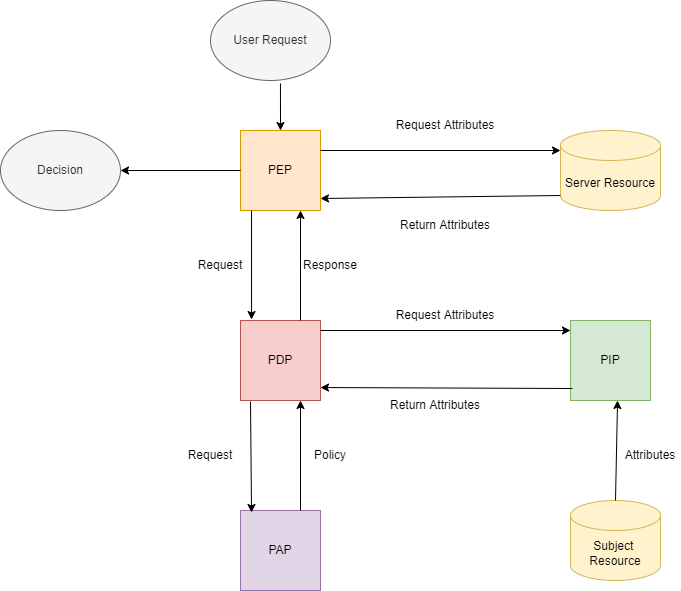
\includegraphics[scale=0.7]{chap2/images/abac.png}
    \caption{architecture de fonctionnement d'ABAC}
	 \label{figAbac}
\end{figure}

User request : est l'utilisateur qui émet une demande \\
Decision : est le résultat qui en ressort du traitement de la demande de l'utilisateur. Elle peut être l'accès accordé ou refusé.\\
Server Resource : est le serveur des applications et des ressources ciblées par la demande de l'utilisateur.\\
Subject Resource : est le serveur des applications et des sources externes.\\
PAP (Policy Administration Point): il est l'endroit où les politiques de contrôle d'accès sont éditées.\\
PEP (Policy Enfoncement Point) : il est responsable de la protection des applications et des données\\ auxquelles on souhaite appliquer ABAC. Il inspecte la demande et génère une demande d'autorisation à partie de celle-ci qu'il envoi au PDP.\\
PDP (Policy Decision Point) : il est le cerveau de l'architecture. C'est l'élément qui évalue les demandes entrantes par rapport aux politiques avec lesquelles il a été configuré. Le PDP renvoie une décision d’autorisation/refus au PEP. Il peut également utiliser des PIP pour récupérer les méta données manquantes.\\
PIP (Policy Information Point) : est le point où le PDP se connecte aux sources externes d'attributs comme LDAP ou une base de données. L'idée est que lors de l'évaluation d'une requête conte une politique, le PDP a besoin d'information (attributs) supplémentaire pour obtenir une décision.

\mySubSection{Avantages du modèle ABAC}{}\label{sectionAvantagesABAC}

\paragraph{} Les systèmes ABAC sont capables d'appliquer à la fois les concepts de contrôle d'accès discrétionnaire (DAC) et de contrôle d'accès obligatoire (MAC). ABAC permet un contrôle d'accès précis, ce qui permet un plus grand nombre d'entrées discrètes dans une décision de contrôle d'accès, fournissant un plus grand ensemble de combinaisons possibles de ces variables pour refléter un ensemble plus grand et plus définitif de règles possibles pour exprimer les politiques.
\paragraph{} Les politiques de contrôle d'accès qui peuvent être mises en œuvre dans ABAC ne sont limitées que par le langage de calcul et la richesse des attributs disponibles. Cette flexibilité permet au plus grand nombre de sujets d'accéder au plus grand nombre d'objets sans spécifier les relations individuelles entre chaque sujet et chaque objet. Par exemple, un sujet se voit attribuer un ensemble d'attributs de sujet lors de son embauche (par exemple, Nancy Smith est une infirmière praticienne dans le service de cardiologie.). Un objet se voit attribuer ses attributs d'objet lors de sa création (par exemple, un dossier contenant des dossiers médicaux de patients cardiaques.). Les objets peuvent recevoir leurs attributs soit directement du créateur, soit à la suite d'outils d'analyse automatisés. L'administrateur ou le propriétaire d'un objet crée une règle de contrôle d'accès en utilisant les attributs des sujets et des objets pour régir l'ensemble des capacités autorisées (par exemple, toutes les infirmières praticiennes du service de cardiologie peuvent consulter les dossiers médicaux des patients cardiaques.). 
\paragraph{} Dans le cadre d'ABAC, les décisions d'accès peuvent changer d'une demande à l'autre en modifiant simplement les valeurs des attributs, sans qu'il soit nécessaire de modifier les relations sujet/objet définissant les ensembles de règles sous-jacents. Cela offre une capacité de gestion du contrôle d'accès plus dynamique et limite les exigences de maintenance à long terme des protections d'objets. 
\paragraph{} En outre, l'ABAC permet aux propriétaires ou aux administrateurs d'objets d'appliquer une politique de contrôle d'accès sans connaissance préalable du sujet spécifique et pour un nombre illimité de sujets susceptibles de nécessiter un accès. Lorsque de nouveaux sujets rejoignent l'organisation, il n'est pas nécessaire de modifier les règles et les objets. Tant que le sujet se voit attribuer les attributs nécessaires pour accéder aux objets requis (par exemple, tous les infirmiers praticiens du service de cardiologie se voient attribuer ces attributs.), aucune modification des règles ou des attributs d'objets existants n'est nécessaire. Cet avantage est souvent appelé "adaptation à l'utilisateur externe (non prévu)", et constitue l'un des principaux avantages de l'utilisation d'ABAC.

\mySubSection{Inconvénient du modèle ABAC}{}\label{sectionInconvénientsABAC}

\paragraph{} Lorsqu'elles sont déployées à l'échelle d'une entreprise dans le but d'accroître le partage d'informations entre diverses organisations, les mises en œuvre d'ABAC peuvent devenir complexes et s'appuyer sur l'existence d'une infrastructure de gestion des attributs, de politiques applicables par les machines et d'un ensemble de fonctions qui prennent en charge les décisions d'accès et l'application des politiques. 
\paragraph{} Outre les exigences de base en matière de politiques, d'attributs et de mécanismes de contrôle d'accès, l'entreprise doit prendre en charge des fonctions de gestion pour le développement et la distribution de politiques d'entreprise, d'identités d'entreprise et d'attributs de sujets, le partage d'attributs de sujets, les attributs d'objets d'entreprise, l'authentification et le déploiement et la distribution de mécanismes de contrôle d'accès. Le développement et le déploiement de ces capacités nécessitent l'examen attentif d'un certain nombre de facteurs qui influenceront la conception, la sécurité et l'interopérabilité d'une solution ABAC d'entreprise. Ces facteurs peuvent être résumés autour d'un ensemble d'activités : \\
- Établir le dossier commercial pour la mise en œuvre d'ABAC \\
- Comprendre les exigences opérationnelles et l'architecture globale de l'entreprise\\
- Établir ou affiner les processus d'affaires pour soutenir ABAC.\\
- Développer et acquérir un ensemble de capacités interopérables.\\
- Opérer avec efficacité\\


\mySection{Politiques et modèles de contrôle d'accès basés sur les rôles attribués}{}\label{sectionAR-BAC}

Le contrôle d'accès basé sur les rôles (RBAC) comme nous l'avons vu dans la littérature est bien connu en raison de sa haute sécurité et de sa facilité de gestion des permissions. Cependant, il présente également certaines lacunes comme la complexité de la structuration des rôles et l'absence de comportement dynamique. Le contrôle d'accès basé sur les attributs (ABAC) est quant à lui un modèle de contrôle d'accès dynamique qui permet de structurer facilement les rôles. Mais son principal inconvénient est que l'analyse des rôles et des permissions après la mise en œuvre du modèle de contrôle d'accès et sa gestion ne sont pas facile dans ABAC. De ce fait, pour pallier aux lacunes de ces deux modèles, il est mis sur pieds un modèle de contrôle d'accès dit hybride baser sur les rôles attribués. Ce modèle met en œuvre et exploite les attributs des objets, des permissions, des rôles et des utilisateurs comme base. De plus, il utilise la capacité de structuration des rôles d'ABAC et le comportement de sécurité stricte de RBAC . Ce modèle est divisé en deux parties :\\
- Dans la première partie du modèle, les permissions automatiques sont créées.\\
- Dans la deuxième partie, les rôles sont automatiquement attribués aux utilisateurs.\\
De manière fondamentale, ce modèle utilise le concept d'attribut, c'est-à-dire qu'il attribue les permissions aux rôles, et puis attribue les rôles aux utilisateurs sur la base des attributs.

\mySubSection{Création automatique des permissions en fonction des niveaux d'action et des conteneurs d'objet}{}\label{sectionCreationPermissionAR-BAC}

Dans ce modèle, les permissions sont automatiquement créées en fusionnant les conteneurs d'objets et les niveaux d'action. Une permission est créée lorsqu'un objet et une action sont combinés ensemble. Le modèle contient les différents niveaux de sécurité et chaque niveau de sécurité a des actions spécifiques. Le niveau 1 comporte des actions de lecture, d'écriture, de modification et de suppression. Le niveau 2 comporte des actions de lecture, d'écriture, de modification, comme le montre la figure. Ces niveaux d'action ont été conçus en fonction de la structure organisationnelle, et d'autres niveaux peuvent être crées par l'administrateur si nécessaire. De même les conteneurs d'objets ont été créés pour le stockage des objets. Différents conteneurs peuvent être créé pour le stockage. Les objets sont affectés aux conteneurs sur la base des types d'objets. Lorsque les objets sont affectés à des conteneurs, le conteneur s'applique à un niveau d'action. Ce processus génère automatiquement un certain nombre de permissions.

\begin{figure}[h!]
    \centering
		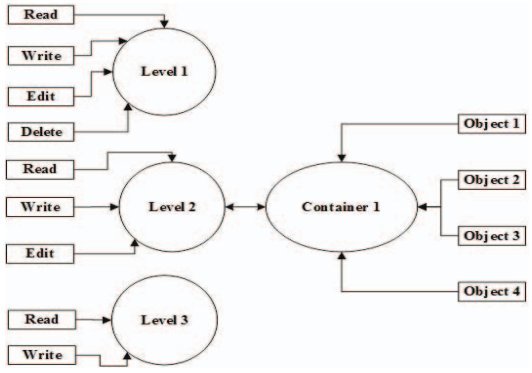
\includegraphics[scale=0.7]{chap2/images/permissionauto.png}
    \caption{création automatique des permissions}
	 \label{figCreationAutoPer}
\end{figure}

Dans la figure, le conteneur 1 qui contient quatre objets s'applique au niveau d'action 2 et le niveau d'action 2 a trois actions, sept permissions sont automatiquement générées. La raison de la création des différents niveaux d'accès est de donner un accès contrôlé aux objets. Chaque fois qu'un objet est créé, les auteurs lui attribuent certaines actions spécifiques comme la lecture et l'écriture uniquement. Certains objets sont génériques. Un objet est créé avec l'attribution d'attribut d'objet comme l'heure, l'adresse IP, le propriétaire. Les attributs des objets sont automatiquement assignés aux permissions, et les permissions contiennent les mêmes attributs que les objets. Les autorisations sont dynamiques et tout changement dans les attributs de l'objet affectera les attributs de l'autorisation. Aucune mise à jour manuelle des autorisations n'est nécessaire dans ce modèle, car l'ajout d'attribut dans le domaine le rend dynamique, facilitant ainsi la création d'autorisations en raison de l'ajout d'attributs, tout en étant robuste et facile à gérer pour les utilisateurs .

\begin{figure}[h!]
    \centering
		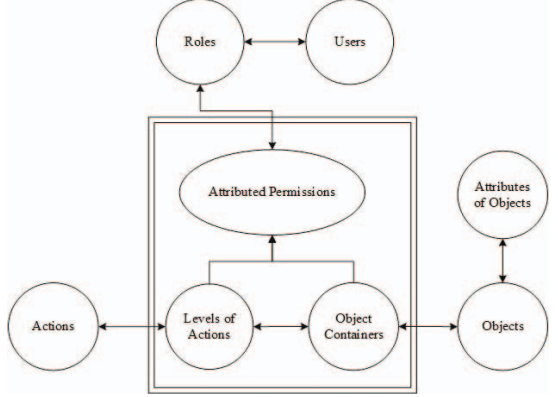
\includegraphics[scale=0.7]{chap2/images/roleAttribue.png}
    \caption{permissions attribuées dans le modèle RBAC}
	 \label{figPermissionAttribué}
\end{figure}
 
\mySubSection{Attribution automatique des permissions aux rôles à l'aide des attributs}{}\label{sectionAttributionAutoAR-BAC}

Ici, les permissions sont attribuées aux rôles automatiquement en utilisant les attributs des objets. Dans le modèle RBAC classique, les autorisations sont attribuées manuellement par l'administrateur, ce qui représente un travail fastidieux pour ce dernier. La structuration des rôles dans RBAC est très difficile. Ici, les critères d'attribution des permissions sont automatiques, ce qui réduit la charge de l'administrateur après la création automatique des permissions, les permissions sont attribuées aux rôles et la décision d'attribution des permissions est prise à l'aide d'expression d'attributs.
\paragraph{} Lorsque les autorisations sont créées automatiquement, elles sont automatiquement attribuées aux rôles comme le montre la figure 5. L'attribution des permissions aux rôles sera faite en utilisant les attributs de permissions. Les rôles sont attribués de la manière suivante : au moment de la création des rôles, l'administrateur définit les attributs du rôle et l'attribution des permissions aux rôles sera effectuée en faisant correspondre ces attributs. Par exemple : un rôle est créé avec l'attribut adresse IP qui a la valeur de 192.168.1.1 et les permissions qui ont la même valeur que l'adresse IP sont attribuées automatiquement à ce rôle .

\begin{figure}[h!]
    \centering
		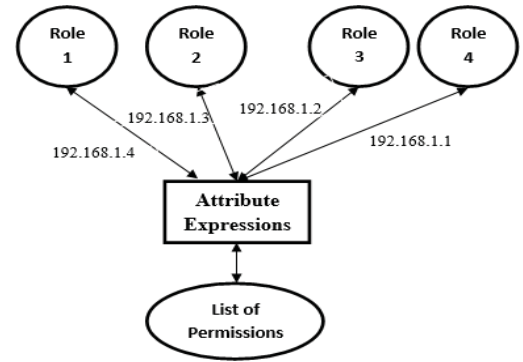
\includegraphics[scale=0.7]{chap2/images/rolepermissionauto.png}
    \caption{Affectation des permissions aux rôles}
	 \label{figPermissionRole}
\end{figure}

\mySubSection{Domaines d'application}{}\label{sectionDomaineApplicationAR-BAC}

Ce modèle peut être appliqué dans le domaine commercial comme l'est RBAC dans les systèmes distribués, dans les nuages tout comme ABAC dans le domaine de la santé, de l'éducation et dans des bases de données. 


\mySubSection{Inconvénients}{}\label{sectionInconvéniantAR-BAC}

Ce modèle ne gère pas les permissions conflictuelles. Et tout comme RBAC et ABAC, il fait confiance à l'administrateur. Ce qui entraîne la création d'entités virtuelles par ce dernier.


\mySection{Politiques et modèles de contrôle d'accès basés sur les rôles améliorés par les attributs(AERBAC)}{}\label{sectionAERBAC}

Qasim Mahmood Rajpoot et Al \cite{rajpoot15}  proposent un modèle de contrôle d'accès qui fournit un mécanisme de contrôle d'accès à grain fin qui non seulement prend en compte les informations contextuelles lors de la prise de décision de contrôle d'accès, mais convient également aux applications où l'accès aux ressources est contrôlé en exploitant le contenu des ressources dans la politique. Ce modèle est la combinaison des deux modèles les plus populaires dans le domaine du contrôle d'accès, l'un étant le modèle de contrôle d'accès basé sur les rôles (RBAC) qui est réputé pour sa simplicité et sa facilité de révision des permissions attribuées à un utilisateur et par sa capacité à rendre la tâche moins lourde à un administrateur. Cependant, il n'est pas adéquat pour les situations où les attributs contextuels sont des paramètres requis pour accorder l'accès à un utilisateur. Une autre limite de RBAC est que les permissions sont spécifiées en terme d'identifiant d'objets, se référant à des objets individuels. Cela n'est pas adéquat dans les situations où un grand nombre d'objets, par centaines de milliers existent et conduit à un problème d'explosion des rôles et des permissions. L'autre étant le modèle de contrôle d'accès basé sur les attributs (ABAC) qui est considéré comme étant plus flexible que RBAC, car il peut facilement prendre en compte les attributs contextuels comme paramètres de contrôles d'accès. Toutefois, ABAC est généralement beaucoup plus complexe que RBAC en termes de révision des politiques, donc l'analyse de la politique et la révision ou la modification des permissions des utilisateurs sont des tâches assez lourdes dans ABAC \cite{rajpoot15}.
\paragraph{} Le modèle que proposent les auteurs conserve la flexibilité offerte par ABAC, tout en conservant les avantages de RBAC, à savoir une administration, une analyse des politiques et une révision des permissions plus facile. En plus de cela, il présente les caractéristiques clé suivantes \cite{rajpoot15} :\\
	-Il permet de prendre des décisions de contrôle d'accès en fonction du contexte en associant des conditions aux permissions qui sont utilisées pour vérifier si les informations contextuelles requises sont présentes au moment de la prise de décision.\\
	-Il offre un système d'autorisation basé sur le contenu tout en gardant l'approche orientée rôle, afin de conserver les avantages offerts par RBAC. Ceci grâce à la spécification des permissions à l'aide des attributs des objets plutôt qu'en utilisant uniquement leur identifiant.


\mySubSection{Composants du modèle AERBAC}{}\label{sectionComposantAERBAC}

Ici les entités utilisateurs, rôles, objets, et opérations ont la même sémantique que dans RBAC. Les utilisateurs et les objets sont également associés à des attributs. L'attribut environnement est également incorporé pour rendre compte de la situation dans laquelle l'accès doit être autorisé . En plus de ceux-là, il intègre des composants tels que \cite{rajpoot15} :

\myDescription{Les attributs }{ils capturent les propriétés d'entités spécifiques (par exemple, l'utilisateur), une fonction d'attribut est définie pour chaque attribut, cette fonction renvoie la valeur de cet attribut. Chaque attribut est représenté par une plage d'ensemble fini des valeurs automatiques. Par exemple, la plage de l'attribut branche est un ensemble de valeurs de noms de branches semi-pertinents pour le domaine d'application. Les attributs utilisateur capturent les propriétés de l'utilisateur qui initie une demande d'accès. Exemple : titre, spécialisation. Les attributs d'objet sont utilisés pour définir les propriétés des ressources protégées par le politique de contrôle d'accès. Exemple : le type, le statut, l'emplacement. Les attributs d'environnement capturent les facteurs externes de la situation dans laquelle l'accès à lieu. Exemple : la température. Un attribut peut être statique, c'est-à-dire que ses valeurs changent rarement, par exemple : la désignation, le département, le type. Soit dynamique, c'est-à-dire que ses valeurs peuvent changer fréquemment et de manière imprévisible, de sorte qu'elles peuvent très bien changer pendant la durée de vie d'une session. Exemple : officier commandant, le lieu, l'occurrence d'un indice.
}

\myDescription{Permissions et conditions }{contrairement aux approches traditionnelles de RBAC, les permissions dans AERBAC font référence aux objets indirectement, en utilisant leurs attributs. Une permission fait référence à un ensemble d'objets partageant des attributs communs, par exemple : le type ou la branche, en utilisant une seule permission, contrairement aux permissions séparées pour chaque objet unique. Ceci est particulièrement pertinent dans les domaines où plusieurs objets partagent des valeurs d'attributs communes. Cela permet de réduire considérablement le nombre d'autorisations associées à un rôle, tout en augmentant l'expressivité et la granularité du contrôle d'accès d'une manière centrée sur les rôles. Dans AERBAC, une permission est constituée d'une expression d'objet et d'une opération autorisée sur l'ensemble d'objets désignés par l'expression. Les expressions d'objet sont formées en utilisant les attributs des objets. Chaque permission est associée à une ou plusieurs conditions, qui doivent être évaluées comme étant vraies pour que l'utilisateur puisse exercer cette permission. Une condition associée à une permission peut contenir les attributs de toutes les entités, y compris les utilisateurs, les objets et l'environnement. Dans certaines applications, il est nécessaire de comparer les attributs des utilisateurs et des objets .
}

\myDescription{Session}{une session contient une liste de permissions associées aux rôles activés par l'utilisateur. Comme décrit précédemment, les permissions sont différentes des permissions RBAC standard en termes de référence aux objets en utilisant leurs attributs et en étant liées aux conditions qui sont évaluées chaque fois qu'une permission doit être exercée. Par conséquent, la fonction checkAccess doit être redéfinie.
}

\myDescription{Demande d'accès}{Dans AERBAC, la demande de l'utilisateur peut également être basée sur les attributs des objets. Par exemple, dans une application d'imagerie médicale, un utilisateur peut vouloir voir toutes les images contenant des caractéristiques spécifiées, par exemple, les objets avec type= tumeur, domaine= hopital-nw. Pour qu'une demande de l'utilisateur soit acceptée, il doit exister une expression d'objet dans la session de l'utilisateur qui désigne les objets demandés, et la condition liée à cette expression d'objets doit être évaluée comme étant vraie. 
}

\begin{figure}[h!]
    \centering
		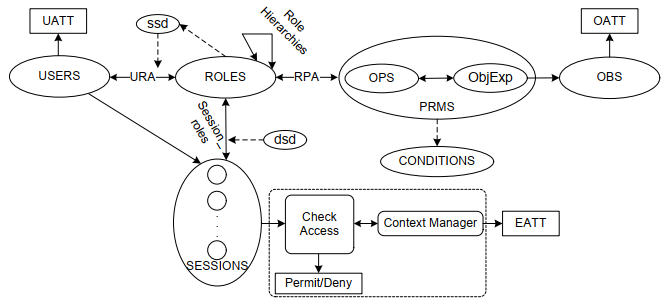
\includegraphics[scale=0.7]{chap2/images/aerbac.png}
    \caption{modèle de contrôle d'accès basé sur les rôles et amélioré par les attributs}
	 \label{figAERBAC}
\end{figure}

\mySubSection{Modèle formel AERBAC}{}\label{sectionModèleAEBAC}

AERBAC est un modèle formel qui incorpore les attributs de l'utilisateur, de l'objet, et de l'environnement dans RBAC d'une manière orientée rôle. La logique de premier ordre est utilisée ici pour faire des descriptions formelles et la convention selon laquelle toutes les variables non liées sont universellement quantifiées et données comme Range (att) est suivi. UATT, OATT et EATT sont respectivement des ensembles de fonctions d'attribut pour les utilisateurs, les objets et l'environnement. Chaque fonction d'attributs renvoie soit un ensemble de valeur, soit une valeur atomique, déterminé en fonction du type de l'attribut (c'est-à-dire attType) \cite{rajpoot15}. 
La relation d'attribution de rôles et de permissions (RPA) capture les permissions qui sont attribuées à un rôle lorsqu'un ensemble donné de conditions est rempli. Un ensemble de permissions peut changer pour un rôle si les conditions varient entre les requêtes. 


\mySubSubSection{Décision d'accès}{}

Dans ce modèle, une demande d'accès de l'utilisateur peut spécifier explicitement un objet, en lisant son identifiant, soit designer implicitement un ensemble d'objet en utilisant les attextributs des objets. Si une demande de l'utilisateur ne porte pas sur un objet spécifique, mais plutôt sur un ensemble d'objets, le système doit prendre en compte les critères donnés pour renvoyer les objets demandés. Lorsqu'un utilisateur soumet une demande d'accès, celle-ci doit être évaluée par rapport à la politique . Nous distinguons ainsi deux formes d'évaluation des demandes selon leur spécification \cite{rajpoot15}.


\myDescription{Demande basée sur l'identifiant}{Ici, l'utilisateur spécifie l'identifiant de l'objet auquel il veut accéder. L'évaluation de ce type de demande est très simple. Dans ce cas, la fonction CheckAccess renvoie true si et seulement s'il existe une permission P dans les permissions disponibles au cours d'une session donnée qui contient une expression d'objet qui vaut vrai pour obj, une opération accordée dans la session et la condition correspondant vaut true. 
}

\myDescription{Demande basée sur les attributs}{Ici, l'utilisateur peut spécifier les attributs de l'objet dans sa demande, plutôt qu'un identifiant unique de l'objet.  Le fait de spécifier les attributs de l'objet dans la demande implique que l'utilisateur souhaite accéder à tous les objets qui ont les valeurs d'attribut spécifiées. Il a donc été examiner deux possibilités de formuler et de traiter de telles demandes. \\
- Requêtes de ressources : Dans cette approche, la demande de l'utilisateur contient une expression similaire aux expressions des objets. La fonction checkAccess reçoit en entrée la demande d'accès et renvoie en sortie les objets autorisés à l'utilisateur si la demande est acceptée, sinon la demande est refusée. L'expression donnée est convertie en une requête et les objets résultants sont récupérés dans la base de données des ressources. L'étape suivante consiste à trouver les expressions d'objet applicables en faisant une comparaison entre l'opération demandée par l'utilisateur et celles mentionnées dans l'ensemble de permissions existantes dans la session de l'utilisateur. Une fois les expressions d'objets sélectionnées, elles sont évaluées une par une pour chaque objet renvoyé par la requête. Si une expression d'objet et sa condition correspondante sont évaluées comme vrai pour un objet, l'objet est ajouté à la liste des objets autorisés à accorder à l'utilisateur. Enfin, l'utilisateur se voit accorder l'accès à tous les objets pour lesquels une expression d'objet et sa condition correspondante sont vraies. Comme les expressions d'objet doivent être évaluées pour chaque objet retourné, cette approche peut s'avérer coûteuse dans le cas où plusieurs objets seraient retournés par la requête formée sur la base de la demande de l'utilisateur. \\
- Les valeurs des attributs : une autre stratégie consiste à évaluer la demande de l'utilisateur par rapport aux expressions d'objets avant de récupérer les objets réels dans la base de données des ressources. Dans cette approche, plutôt que de fournir une expression, l'utilisateur spécifie sa demande d'accès en indiquant les valeurs d'attribut des objets souhaités. La fonction checkAccess reçoit en entrée la demande Req de l'utilisateur et renvoie les objets désignés par les valeurs d'attributs d'objets données dans Req, si la demande est acceptée, sinon la demande est refusée. Pour traiter la demande de l'utilisateur, on identifie toutes les expressions d'objet existant dans la session de l'utilisateur qui utilisent les attributs mentionnés dans la demande de l'utilisateur et l'opération spécifiée dans cette permission correspond à l'opération demandée. Les expressions d'objet qui incluent un attribut non spécifié par la demande de l'utilisateur ne sont pas pertinentes. Ensuite, pour chaque expression d'objet pré-sélectionnée, les fonctions d'attribut dans l'expression d'objet reçoivent les valeurs d'attribut fournies par l'utilisateur. Dès qu'une expression d'objet et sa condition correspondante reviennent à la réalité, la demande de l'utilisateur est acceptée et les autres expressions d'objet sont ignorées. Lorsqu'une expression retourne vraie, il est formé une requête basée sur les valeurs d'attributs d'objets spécifiées dans la demande de l'utilisateur et l'utilisateur a accès à tous les objets retournés par la requête. \\
Ici ne sont évaluées que les expressions d'objet qui utilisent des attributs d'objet spécifiés dans la requête de l'utilisateur. \\
Cette approche permet de prendre une décision d'accès en évaluant uniquement les expressions d'objet, sans avoir à extraire les objets de la base de données des ressources. C'est important, car de nombreuses demandes peuvent être refusées à ce stade sans avoir à récupérer les objets et à évaluer les conditions. 
}

\mySubSection{Inconvénients}{}\label{sectionInconvéniantARBAC}

Tout comme ses prédécesseurs, ce modèle octroie tout le pouvoir au DBA d'une organisation en lui faisant une totale confiance. Ce qui n'est pas très normal, car ce dernier, parfois, use de ce pouvoir pour faire du n'importe quoi dans le système.

\mySection{Politiques et modèles de contrôle d'accès basés sur les rôles et les attributs(ARBAC)}{}\label{sectionARBAC}
 
 C'est dans le but de résoudre le problème d'explosions de rôles et des permissions que soulève RBAC et celui de la difficulté d'analyser le politiques de sécurité que soulève ABAC que Singh et al, ont proposé en modèle de contrôle d'accès qui définie les politiques de sécurité sur la base des rôles et des attributs (ARBAC). ARBAC introduit au dessus du modèle RBAC le concept de "règle"  qui est basée sur les attributs. il associe les règles à des rôles et des permission afin de permettre le spécification des politiques multidimensionnelles à grain fin \cite{singh19}.
 
\mySubSection{Composants du modèle ARBAC}{}\label{sectionComposantARBAC}

\myDescription{User ou Utilisateur}{un utilisateur est une entité qui provoque le flow d'information et est capturée par la relation \textit{User}. Les utilisateurs peuvent avoir un ou plusieurs attributs, et chaque attribut peut avoir une ou plusieurs valeurs d'attribut qui sont capturés dans les relations \textit{User-attribute} et \textit{User-attribute-values} respectivement \cite{singh19}.}

\myDescription{Objet}{Dans une organisation, les objets contiennent ou reçoivent des informations et sont capturés dans la relation \textit{Objet}. Les objets peuvent avoir un ou plusieurs attributs, et chaque attribut peut avoir une ou plusieurs valeurs d'attribut qui sont capturés dans les relations \textit{Object-attribute} et \textit{Object-attribute-values} respectivement \cite{singh19}.}

\myDescription{Environnement}{L'environnement tel que le temps, l'emplacement est un facteur supplémentaire, indépendant de l'utilisateur et de l'objet, qui peut restreindre d'avantage la disponibilité des objets pour les utilisateurs. il peut avoir un ou plusieurs attributs et chaque attribut peut avoir une ou plusieurs valeurs qui sont saisie dans les les relation \textit{environment-attribute} et \textit{enivronment-attribute-values} respectivement \cite{singh19}.}

\myDescription{Rôles et hiérarchie des rôles}{les rôles définissent les fonctions professionnelles que les utilisateurs supposent exécuter dans une organisation. Une rôle dans ARBAC, est contraint par un ensemble de règles qui peuvent être composées d'attributs d'utilisateur et d'attributs de l'environnement. Ainsi les rôles seraient disponibles que pour les utilisateurs qui possèdent les attributs nécessaires et satisfont au moins une des règles associées à ces rôle. la hiérarchie des rôles définie une relation d'ordre partiel sur les rôles qui permet l'héritage des rôles \cite{singh19}.}

\myDescription{Permission}{Une permission définie l'autorisation sous la forme d'un droit (Par exemple, lecture, écriture, etc.) sur un objet qui habilite un utilisateur à effectuer une tâche par le biais d'un rôle.}

\myDescription{Attribution des rôles aux utilisateurs}{Ici un utilisateur peut avoir un ou plusieurs rôles, et un rôle peut être attribué à plusieurs utilisateurs.}

\myDescription{Affectation des permissions aux rôles}{Dans ARBAC, un rôle peut avoir une ou plusieurs permissions, et une permissions peut être assignée à plusieurs rôles.}

\myDescription{Session}{Dans RBAC, une session capture un sous-ensemble de rôles actifs de l'ensemble des rôles attribués à un utilisateur. un utilisateur peut activer une ou plusieurs sessions, mais chaque session serait attribuéeà un seul utilisateur. Dans ARBAC, l'activation d'un sous-ensemble de rôles d'utilisateur dans des sessions dépendant de la satisfaction des règles à ces rôles \cite{singh19}. }

\myDescription{Contraintes}{L'ARBAC proposé peut également spécifier différents types de contraintes qui permettent de capturer les rôles ou les permissions critiques d'une organisation, le lien entre l"utilisateurs et un rôle ou celui entre un rôle et une permission, les valeurs d'attribut communes à un ensemble d'utilisateurs ou d'objets et en fin la relation cardinalité qui permet de voir le nombre d'occurrences de chaque relation. }

\myDescription{Règle}{ARBAC introduit la notion de règle afin d'activer ou de déactiver les rôles et les permissions. 
\paragraph{} Dans l'ARBAC, les règles qui restreignent la disponibilité des rôles pour les utilisateurs peuvent être composées des valeurs d'attributs d'utilisateur et de valeurs d'attributs d'environnement .
De même, les règles qui restreignent la disponibilité des permissions peuvent être composées de valeurs d'attribut d'utilisateur, de valeurs d'attribut d'objet, et de valeurs d'attributs d'environnement \cite{singh19}.
}

\myDescription{Attribution des règles aux rôles}{RuR dans ARBAC, capture l'association des règles aux rôles. Une règle peut être assignée à plusieurs rôles, et un rôle, peut avoir plusieurs règles. L'association d'un ensemble de règles basées sur les attributs à chaque rôle permet de réduire l'espace des règles applicables pour un rôle, et de minimiser le temps d'évaluation de la disponibilité des rôles pour un utilisateur \cite{singh19}.}

\myDescription{Attribution des règles aux permissions}{RuP dans ARBAC, capture l'association des règles avec les permissions. Une règle peut être assignée à plusieurs permissions, et une permissions, peut avoir plusieurs règles. L'association directe d'un ensemble de règles basées sur les attributs aux permissions permet de réduire l'espace des règles applicables pour une permission, et de minimiser le temps d'évaluation de la disponibilité de la permission pour un rôle \cite{singh19}.}

\mySubSection{Avantages du modèle ARBAC}{}\label{sectionAvantageARBAC}

Comme avantages: \\
- le modèle ARBAC permet une administration plus facile des politiques.\\
- il permet de limiter la disponibilité des rôles et des permissions.\\
- ce modèle permet une spécification de politiques flexibles et sensibles au contexte. C'est-à-dire que grâce aux concepts de règle, d'attribut et d'environnement qu'introduit ARBAC nous permettent d'exprimer des politiques d'accès basées sur des attributs et ceci dans un contexte bien précis.\\
- ce modèle permet de minimiser considérablement les effets de migration. En effet, cette approche permet aux entreprises et applications utilisant le modèle RBAC de migré leurs politiques dans ARBAC sans toutes fois les modifier

\mySubSection{Inconvénients du modèle ARBAC}{}\label{sectionInconvenientARBAC}

Comme inconvénients nous avons: \\
- ARBAC ne permet pas l'analyse automatique de la sécurité des politiques.\\
- ce modèle ne permet pas de contrôles les faits et gestes du super-utilisateur
 
 
\mySection{Politiques et modèles de contrôle d'accès basés sur la hiérarchie organisationnelle (HOr-RBAC)}{}\label{sectionHOrRBAC}

Les politiques basées sur la hiérarchie organisationnelle sont venues palier au problème des politiques précédentes. Elles permettent d'exprimer les règles de sécurité telles que \cite{theseBenoit} : \\  
- Les règles qui spécifient le contrôle du super-utilisateur \\
- Les règles qui spécifient la hiérarchie entre les unités administrative et opérationnelles \\
- Les règles spécifiques pour empêcher l'ajout des entités virtuelles dans le système d'information d'une organisation 
\paragraph{} HOr-BAC s'appuie sur le modèle Or-BAC en y implémentant des concepts propres à lui-même. Ces politiques tirent leur originalité du fait qu'elles sont purement construites autour de la structure organisationnelle d'une organisation, cela signifie que dans le modèle HOr-BAC, il est possible pour nous de trouver tous les composants principaux de la structure organisationnelle d'une organisation réelle.

\mySubSection{Composants de base du modèle HOr-BAC}{}\label{sectionComposantHOr-BAC}

\myDescription{L'unité organisationnelle}{C'est un regroupement des unités administratives et opérationnelles. Elle est définie dans notre modèle comme une entité ayant un rôle administratif ou opérationnel et remplace ainsi l'entité rôle vu dans le modèle Or-BAC. Ce concept nous permet de mieux représenter la relation hiérarchie qu'il existe entre ces deux unités \cite{theseBenoit}. \\
- L'unité opérationnelle : elle représente l'ensemble des employés métiers ayant les mêmes formations, les mêmes rôles et une fonction spécifique dans une organisation. Elle ne prend aucune décision sur le fonctionnement de l'organisation et ne fait qu'obéit aux décisions qui lui ont été données par l'unité administrative qui la subordonne. Exemple : comptabilité, enseignant. \\
- L'unité administrative : elle représente l'ensemble des unités décisionnelles de l'organisation. Cette entité permet de représenter les fonctions de contrôle, de supervision, et de validation des requêtes émises dans le SI. Elle peut être placée sur une unité opérationnelle ou sur une autre unité administrative. Exemple : département, rectorat et décanat dans une université. Les modèles précédents basés sur les rôles n'ont pas fait une différence entre un rôle opérationnel et un rôle administratif. Or, il existe bel et bien une différence entre ces rôles. En considérant par exemple les rôles,  directeur et infirmier dans une organisation hospitalière, ils ne sont pas de même nature, car l'infirmier travaille sous le contrôle du directeur ; Ainsi, le rôle infirmier est une unité opérationnelle et le rôle directeur est une unité administrative.
}
\myDescription{Employé métier}{Il représente une personne physiquement identifiable ayant un rôle actif dans l'organisation. C'est la seule entité réellement active dans l'organisation. Le concept d'employé métier remplace le concept de sujet vu dans le modèle Or-BAC. L'intérêt d'une telle approche réside sur le fait qu'étant donné que l'utilisateur est une personne physique, il pourra être facilement contrôlé ; Car s'il existe des sujets virtuels, le super-utilisateur pourra les ajouter autant qu'il le souhaite et les habiliter à jouer les rôles de son choix.
}

\myDescription{Les ressources}{
L'entité ressource est utilisée pour organiser l'ensemble des données de l'organisation et exprimer les entités passives. Cette entité peut être la note d'un étudiant, les dossiers d'inscription, les dossiers de changement de grade des enseignants pour une organisation universitaire \cite{theseBenoit}.
}
\myDescription{La requête}{Elle est définie comme étant une demande faite par un Employé métier de l'organisation. Une requête doit avoir les informations suivantes : le nom de l'émetteur et la ressource. Il existe deux types de requêtes à savoir les requêtes à exécution directe (réelle) et indirecte (différée). Lorsqu'elle est indirecte, elle nécessite automatiquement la validation du supérieur hiérarchique. Par contre une requête à exécution directe n'a pas besoin de validation du supérieur hiérarchique.
}

\mySubSection{Mode de traitement d'une requête dans HOr-BAC}{}\label{sectionModeTraitementBOr-BAC}

Il consiste à définir certains attributs qui seront pris en compte lors de l'émission et du traitement d'une requête. Étant donné que l'un des buts du modèle HOr-BAC est le contrôle des opérations de base d'un DBA dans une organisation de manière interactive, nous nous intéresserons sur les attributs suivants : \\
- Effet : consiste à spécifier si la requête émise doit attendre l'accord de la hiérarchie ou pas.\\
- Attente : spécifie le temps d'attente après lequel l'émetteur obtient l'accord tacite de sa requête.\\
- Nombre : spécifie le nombre de fois que l'émetteur a le droit d'exécuter une requête. \\
- Mode : spécifie le mode de traitement de la requête qui peut être validé, rejeté ou transmis.

\mySubSection{Politique de sécurité du modèle HOr-BAC}{}\label{sectionPolitiqueBOr-BAC}

Une politique de sécurité réglemente les accès au système à travers des permissions. Une permission dans notre modèle matérialise le fait qu'une organisation autorise une unité organisationnelle de traiter ou d'émettre une requête donnée dans une vue donnée. Le modèle HOr-BAC  dans le but de matérialiser la hiérarchie entre les différentes unités organisationnelles implémente en son sein deux types de permission afin de différencier les actions effectuées par chaque unité. Ainsi, on distingue donc :\\
- Les permissions dites de préparation : encore appelée permissions opérationnelles. Elles permettent aux unités opérationnelles de préparer (initier, émettre ou soumettre) des requêtes à leur hiérarchie. Cela laisse sous-entendre qu'aucune unité opérationnelle n'a le droit de traiter une requête venant d'une autre unité organisationnelle, car sa seule fonction est d'exécuter. Elle est matérialisée par la relation permissions-opérationnelles qui relie les entités organisation, unité opérationnelle, requête et vue.\\
- Les permissions dites de validations : encore appelées permissions administratives. Elles permettent aux unités administratives de traiter (contrôler, rejeter, valider et/ou transmettre) les requêtes provenant des unités opérationnelles. Elle est matérialisée par la relation permissions-administratives qui relie les entités organisation, unité opérationnelle, unité administrative, requête et vue. \\
Sachant qu'une personne est appelée à jouer au sein d'une organisation un certain nombre de rôles, y compris ceux qu'elle joue habituellement, le modèle HOr-BAC nous donne la possibilité à travers l'entité contexte de définir une situation ou des circonstances dans lesquelles les organisations accordent des permissions à des rôles pour réaliser des requêtes sur des vues. Ainsi à nos permissions citées plus haut nous ajoutons l'entité contexte pour spécifier à quel moment, situation et localisation les unités opérationnelles et administratives sont respectivement appelées à émettre ou à traiter une requête donnée dans une vue donnée. Ces permissions ne permettent qu'à une organisation donnée de spécifier les permissions accordées aux unités organisationnelles suivant un contexte précis. Mais, elles ne permettent pas de  décrire des actions concrètes que réalisent les employés sur les ressources. Ainsi, nous avons implémenté le concept de contrôle d'accès de bas niveau à travers les relations suivantes :\\
- Peut-suggérer : cette relation permet à un employé d'obtenir la permission de suggérer l'application d'une action sur une ressource donnée.\\
- Peut-traiter : cette relation matérialise le fait que le supérieur hiérarchique d'un employé a l'autorisation de traiter les suggestions d'application d'une action donnée sur une ressource donnée.

\mySubSection{Architecture de fonctionnement du modèle HOr-BAC: parapheur électronique}{}\label{sectionArchitectureBOr-BAC}

Contrairement aux autres modèles, le modèle HOr-BAC implémente en son sein le concept de parapheur électronique. Il s'agit ici d'un processus de contrôle de l'émission et du traitement des requêtes dans un système d'information. Il permet de contrôler les actions des utilisateurs du système y compris celles du  super-utilisateur ou DBA. Ici, nous supposons que la quasi-totalité des actions dans une organisation se fait sur la demande et chaque demande obtient une validation pour une exécution effective dans le système sinon, la demande est rejetée. Son fonctionnement est illustré par le schéma ci-dessous :

\begin{figure}[h!]
    \centering
		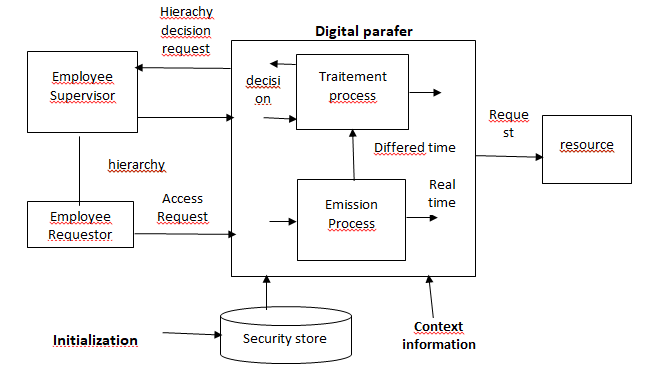
\includegraphics[scale=0.7]{chap2/images/hor-bac.png}
    \caption{composants du parapheur électronique}
	 \label{figHor-bac}
\end{figure} 

Employee Request : c'est l'employé qui émet la requête \\
Employee Supervisor : c'est le supérieur hiérarchique de l'employé qui émet la requête. Il a pour rôle de valider, refuser, traiter ou transmettre la requête de ce dernier.\\
Le security store : il représente la base de données qui stocke les politiques de sécurité de l'entreprise, les informations sur la structure organisationnelle, les informations sur les employés, les comptes utilisateurs. Toutes ces informations sont enregistrées avant le fonctionnement du parapheur.\\  
Initialization : c'est l'ensemble des procédures permettant d'enregistrer les données dans le security store.\\
Context information : c'est le contexte (temporel, géographique, lié au sujet ou à la ressource) dans lequel la requête est traitée.\\
Emission process : c'est l'algorithme qui permet l'émission d'une requête. Selon le type de la requête, il effectue le traitement donné. S'il s'agit d'une requête immédiate, il l'exécute de façon automatique et enregistre son résultat dans la BD avant d'accorder ou pas l'accès à la ressource à ce dernier. Si la requête est différée, il l'enregistre puis la transmet au traitement process.\\
Traitement process : c'est l'algorithme qui s'occupe du traitement des requêtes différées. Quand il reçoit une requête, il envoie une alerte au supérieur hiérarchique de l'employé qui a émis la requête pour qu'il la valide, refuse, traite ou la transmette. Une fois qu'il obtient la décision du supérieur hiérarchique, il accorde ou pas l'accès à la ressource.\\
Resource : c'est la ressource à laquelle un employé souhaite accéder.


\mySubSection{Inconvénient du modèle HOr-BAC}{}\label{sectionInconveniantHOr-BAC}

Dans HOr-BAC, les politiques de contrôle ne peuvent être définies que sur la base de l'unité organisationnelle à laquelle appartient un employé, ce qui limite ainsi la flexibilité du contrôle d'accès. Par conséquent il ne permet que de définir des politiques de contrôle d'accès à gros grain, c'est-à-dire des politiques qui ne sont définies que sur la base des unités organisationnelles. 


\mySection{Conclusion}{}\label{sectionSyntheseChap1}

En somme, nous avons présenté dans ce chapitre l'état de l'art sur les politiques et modèles de contrôles d'accès. Nous avons vu que bien que les politiques et modèles de contrôles d'accès discrétionnaires et obligatoires ont été implantés dans les systèmes d'exploitation Windows et Linux, leur principal inconvénient est que les permissions sont directement affectées aux utilisateurs. Les politiques
et modèles à bases des rôles ont donc vu le jour pour palier à ce problème. Le premier de ces modèles a été le modèle RBAC qui a introduit la notion de rôle dont les permissions sont affectées aux rôles et les rôles affectés aux utilisateurs. Son inconvénient majeur a été l'héritage des rôles. De plus, ce modèle n'exprime pas les permissions et les interdictions. Le modèle Or-BAC est donc venu résoudre ces
problèmes en introduisant le concept d'organisation. Cependant, ces différents modèles permettent d'exprimer les politiques de sécurité de façon statique. Ainsi ABAC a vu le jour. ABAC attribue l'accès aux ressources sur la base des attributs de différentes entités, il permet une spécification flexible des politiques de sécurité et un contrôle à grain fin des ressources du système. Toutefois, ABAC est difficile d'administration. De ce fait, plusieurs auteurs ont proposé différentes modèles issues de la fusion des modèles RBAC et ABAC afin de combler leurs lacunes. l'un de ces modèles fut le modèle de contrôle d'accès basé sur les rôles attribués. Nous avons vu plus haut que, ce modèle permet de créer des façon dynamique les permissions et de les attribuer automatiquement aux rôles. Tout comme RBAC ce modèle est facile à administrer et tout comme ABAC il permet un contrôle d'accès à grain fin. Cependant, ce modèle ne résous pas le problème d'explosion de rôles et de permission donc souffre RBAC. Le modèle de contrôle d'accès basé sur les rôles améliorés par les attributs (AERBAC) vient résoudre ce problème en permettant une flexible des politiques de sécurité basé sur les rôles et attribut. Toutefois d'après \cite{singh19}, AERBAC ne résous pas totalement le problème d'explosion des rôles et des permissions que pose RBAC et modifie pas la même occasion la structure de base de ce dernier. Ainsi ils proposent un nouvelle modèle qui place place au dessus de la structure de base de RBAC le concept de règle basé sur les attributs d'utilisateur, d'objet et de contexte qui permet d'activer ou de désactiver les rôles et les permission. Ce modèle permet également un contrôle à grain fin des objets du système. Mais aucun de ces modèles ne contrôle le super-utilisateur dans un système d'information. Nous avons ainsi vu que c'est le modèle HOr-BAC qui a effectué ce contrôle en intégrant au modèle Or-BAC le concept de parapheur électronique. L'inconvénient majeur du modèle HOr-BAC est que les politiques de contrôle ne peuvent être définies que sur la base de l'unité organisationnelle à laquelle appartient un employé, ce qui limite ainsi la flexibilité du contrôle d'accès.

